\section{Portfolio revision implementation}
The portfolio revision model is an extension of the CVaR model to revise and evaluate portfolios after some time has past.
In this work, is assumed that four weeks are gone and the previous portfolio on section~\ref{sec:CVaR} could no longer be credible and acceptable.
So, a revision of the portfolio on the (2008-03-28) to maximize the return under two different strategies (risk averse and risk neutral) are considered.
The portfolio revision entails some costs for the transactions deviations on the portfolio.
Here, we assume a transaction cost of 0.1\% of the traded amount in kr., and a minimum cost of at least 50 kr per trade.
These costs are taken to be paid from our own pocket outside of the value of the assets.

The portfolio revision model is defined as
\begin{align}
\up{TotalCost} &= \lambda \up{CVaR} - {\left( 1 - \lambda \right)} \up{MeanReturn} + \up{TradeCost} \\
x^\up{old}_{i} + x^\up{difference}_{i} &= x_{i} \; \; \forall i \\
\sum_{i} x^\up{old}_{i} &= \sum_{i} x_{i} \\
x^\up{difference}_{i} &\le B_{i} \up{M} \; \; \forall i \\
-x^\up{difference}_{i} &\le B_{i} \up{M} \; \; \forall i \\
\up{TradeCost} &= \sum_{i} \up{TC}_{i} \\
\up{TC}_{i} &\ge B_{i} \up{penalty} \; \; \forall i \\
\up{TC}_{i} &\ge 0.001 x^\up{difference}_{i} \; \; \forall i \\
\up{TC}_{i} &\ge - 0.001 x^\up{difference}_{i} \; \; \forall i 
\end{align}
where $\lambda$ is the level of risk of the strategy (1 - Risk Averse ; 0 - Risk Neutral), TradeCost is the total cost of the trades of all changes in portfolio, and $x^\up{old}_{i}$ is the previous result of portfolio updated with the current historical monthly return.
In this way, the first $x^\up{old}_{i}$ is based on the results of section~\ref{sec:CVaR} using the risk averse result.
The difference between the $x^\up{old}_{i}$ and the new $x_{i}$ is given by $x^\up{difference}_{i}$.
$B_{i}$ is a binary variable which characterizes if there is or is not a transacation in each ETF $i$, and M is a high constant value to allow the selection of trade or not trade, chosen here to be equal to the value of the portfolio.
$\up{TC}_{i}$ is the trade cost incurred due to trading in each ETF $i$, and penalty corresponds to the trade cost of 50 kr.
In addition to the previous constraints, constraints~\eqref{eq:MeanReturn}~through~\eqref{eq:VarDev} in the CVaR model presented in section~\ref{sec:CVaR} is considered as constraints in the portfolio revision model.

The initial solution is obtained running the full portfolio revision mode where the value of $x^\up{old}_{i}$  is based on the previous results of CVaR model updating with the current historical return (2008-03-26). 
$x^\up{old}_{i}$  is given by
\begin{align}
x^\up{old}_{i} &= x_{i} (1+ r_{i,m})
\end{align}
where $r_{i,m}$ is the histoical monthly return.

\begin{figure}[tpbh]
\centering
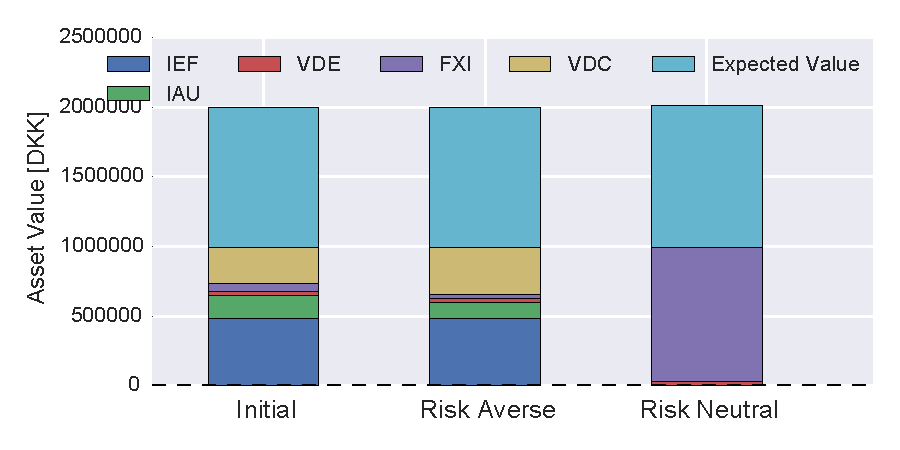
\includegraphics{../pic/portfoliorevision_portfolio.pdf}
\caption{Initial portfolio versus those found by the two types of traders.}
\label{fig:prevpf}
\end{figure}

\begin{table}
\caption{Stats for portfolios found by portfolio revision model.}\label{tbl:portfoliotabel}
\centering
\begin{tabular}{lrrr}
\toprule
{} &  Expected Profit &      CVaR &  Trading Cost \\
\midrule
Type         &                  &           &               \\
Initial      &          8423.76 &   3436.86 &          0.00 \\
Risk Averse  &          6545.42 &   2469.89 &        214.37 \\
Risk Neutral &         24735.63 &  36958.75 &       1820.37 \\
\bottomrule
\end{tabular}

\end{table}

The aim of the present section is to minimize the TotalCost of the full portfolio revision model for each type of strategy (risk averse and risk neutral).
The portfolios are shown on Figure~\ref{fig:prevpf}, while the resulting expected value, CVaR and trading are presented in Table~\ref{tbl:portfoliotabel} considering a comparison between the different strategies and the initial solution. 

The risk-averse strategy makes a small adjustment to the portfolio to decrease the CVaR, while the risk-neutral trader throws away pretty much the entire portfolio to nearly only include a single, high risk asset with high historic return.
Trading a very large value in this way yields a very high trading cost, which is made up for by the large increase in expected profit.